% Drawing 43/10-1 -- folder 43, batch 10, archive page 183 (PDF page 184).
% Transcription: schéma encadré : à gauche $\mathbb{G}_m$, $\mathbb{G}_a$ soulignés ; deux traits en éventail en partent. Sur le trait supérieur : $\mathbb{Z}/\ell\mathbb{Z}$, puis $\mu_p$, $\alpha_p$, $\mathbb{Z}/p\mathbb{Z}$ ; sur le trait inférieur : $\mu_p$, $\alpha_p$, $\mathbb{Z}/p\mathbb{Z}$, puis $\mathbb{Z}/\ell\mathbb{Z}$ ; les deux convergent vers $\mathbb{V}$ et $\mathbb{Z}$ (lettres doublées) soulignés, à droite. Le schéma met face à face, dans l'ordre inverse, les groupes que la page 192 énumère
% Kind: framed schema: two fans of groups from G_m, G_a to V, Z. Method 2 (schematic redraw from the facsimile). Status: ok.
% Notes: In a frame: G_m, G_a underlined at the left; two strokes fanning out; on the upper stroke Z/lZ, then mu_p, alpha_p, Z/pZ; on the lower stroke mu_p, alpha_p, Z/pZ, then Z/lZ; both converge to V and Z (doubled letters) underlined at the right. Two long strokes crossing the frame (crossing out the page) are drawn grey.
% Coordinates: 1 unit = 1 mm = 1/100 of the crop width (bbox in page fractions: [0.05, 0.3, 0.97, 0.55]).
% Redrawn by Claude (claude-opus-5-5), issue #73, 2026-11-07; not checked by a human; not compiled (no TeX in the session).
% Rights: reproduces part of the work -- behind RENDER_TRANSCRIPTS, never published by itself.
\documentclass[tikz,border=3pt]{standalone}
\usepackage{amsmath,amssymb}
\usetikzlibrary{patterns,arrows.meta}
\tikzset{pencil/.style={black!45}, struck/.style={black!35}, mark/.style={circle,draw,inner sep=1.3pt}, pt/.style={circle,fill,inner sep=0.9pt}, opt/.style={circle,draw,fill=white,inner sep=1.1pt}}
\begin{document}
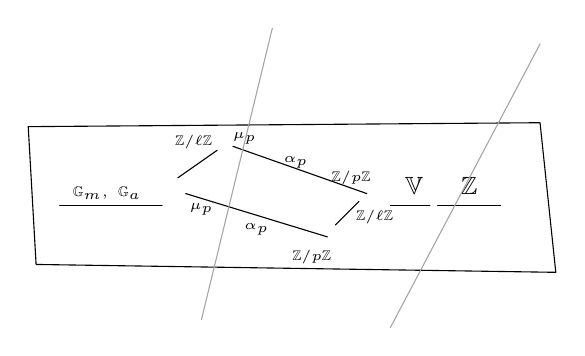
\begin{tikzpicture}[x=1mm,y=1mm,line cap=round,line join=round,font=\scriptsize]
\draw (11,-12.5) -- (76,-12) -- (78,-31) -- (12,-30) -- cycle;
\node[inner sep=1pt] at (21,-21) {\tiny $\mathbb G_m,\ \mathbb G_a$};
\draw (15,-22.5) -- (28,-22.5);
\draw (30,-19) -- (35,-15.5);
\node[inner sep=1pt] at (32,-14.5) {\tiny $\mathbb Z/\ell\mathbb Z$};
\draw (37,-15) -- (54,-21);
\node[inner sep=1pt] at (38.5,-14) {\tiny $\mu_p$};
\node[inner sep=1pt] at (45,-17) {\tiny $\alpha_p$};
\node[inner sep=1pt] at (52,-19) {\tiny $\mathbb Z/p\mathbb Z$};
\draw (31,-21) -- (49,-26.5);
\node[inner sep=1pt] at (33,-23) {\tiny $\mu_p$};
\node[inner sep=1pt] at (40,-25.5) {\tiny $\alpha_p$};
\node[inner sep=1pt] at (47,-29) {\tiny $\mathbb Z/p\mathbb Z$};
\draw (50,-25) -- (53,-22);
\node[inner sep=1pt] at (55,-24) {\tiny $\mathbb Z/\ell\mathbb Z$};
\node[inner sep=1pt] at (60,-20) {\small $\mathbb V$};
\node[inner sep=1pt] at (67,-20) {\small $\mathbb Z$};
\draw (57,-22.5) -- (62,-22.5);
\draw (63,-22.5) -- (71,-22.5);
\draw[struck] (42,0) -- (33,-37);
\draw[struck] (76,-2) -- (57,-38);
\end{tikzpicture}
\end{document}
